%ju 26-Dez-22 10-Kuehlsystem.tex
\textbf{Welche Aufgabe hat das Kühlsystem eines Verbrennungsmotors?}

\begin{enumerate}
\item
  schnelle Erwärmung des Motors auf Betriebstemperatur
\item
  überschüssige Wärme muss schnell und zuverlässig abgeleitet werden
\end{enumerate}

\textbf{Betriebstemperatur}

Kühlmitteltemperaturen zwischen $80 - 120^\circ\text{C}$

Überdruck im Kühlsystem: Pkw: 1,3 -- 2 bar, Nfz: 0,5 -- 1,1 bar (bessere
Kühlung, erfordert Ausgleichsbehälter)

\textbf{Ziel: schnelles Erreichen der Betriebstemperatur des Motors}

$\to$ geringerer Kraftstoffverbrauch und Schadstoffemissionen

\section{Anforderungen an das
Kühlsystem}\label{anforderungen-an-das-kuehlsystem}

\begin{enumerate}
\item
  ausreichende Kühlwirkung
\item
  schnelles Erreichen der Betriebstemperatur
\item
  geringes Gewicht
\item
  gleichmäßige Kühlung der Bauteile, um Wärmespannung zu vermeiden
\item
  geringer Energiebedarf für den Betrieb des Kühlsystems
\end{enumerate}

\emph{Eine gute Kühlung ermöglicht somit} $\dots$

\begin{enumerate}
\item
  verbesserte Zylinderfüllung
\item
  verminderte Klopfneigung bei Ottomotoren
\item
  höhere Verdichtung
\item
  höhere Leistung
\item
  geringerer Kraftstoffverbrauch
\item
  gleichmäßige Betriebstemperaturen
\end{enumerate}

\section{Welche Kühlungsarten werden
unterschieden?}\label{welche-kuehlungsarten-werden-unterschieden}

\begin{enumerate}
\item
  \textbf{Luftkühlung} (Fahrtwindkühlung, Gebläseluftkühlung)

  \begin{itemize}
  \item
    $\to$ Wärme wird direkt an die umströmende Umgebungsluft abgegeben
  \item
    Nachteil: größere Schwankungen der Betriebstemperatur
  \end{itemize}
\item
  \textbf{Flüssigkeitskühlung} (Pumpenumlaufkühlung,
  Zwangsumlaufkühlung)

  \begin{itemize}
  \item
    $\to$ Kühlmittel nimmt die Wärme auf und gibt sie durch den Kühler
    an die Umgebungsluft ab
  \item
    Vorteil: gleichmäßige Kühlwirkung, Motortemperaturregelung
  \end{itemize}
\item
  \textbf{Innenkühlung des Brennraums} (Verdampfung des Kraftstoffs)

  \begin{itemize}
  \item
    $\to$ Energie aufnehmen - aus der Umgebung wird Wärme entzogen.
  \item
    Notwendig, wenn man eine Flüssigkeit verdampfen möchte. (flüssig
    $\to$ gasförmig, Druck ist konstant)
  \end{itemize}
\end{enumerate}

\section{Additive für Kühlmittel}\label{additive-fuer-kuehlmittel}

\begin{itemize}
\item
  Konditioniertes Kühlmittel (Gemisch aus Wasser und Frostschutzmittel -
  bekannt als Glysantin, Ethylenglykolbasis G11/12, Propylenglykolbasis
  G13)
\item
  Korrosionsinhibitoren (Hemmstoff, Schutz vor Korrosion)
\item
  Schutz gegen Kesselstein (Kalkablagerung)
\item
  Neutralisationsmittel gegen Ameisen- und Essigsäure
\item
  Kavitation Schutzmittel (Dampfblasen)
\item
  Antischaumbildner
\end{itemize}

\section{Kavitation (lat. cavitare, aushöhlen, Hohlsog, Abtragen von
Werkstoff)}\label{kavitation-lat.-cavitare-aushoehlen-hohlsog-abtragen-von-werkstoff}

\textbf{Kavitation} wird der Dampfdruck (Mischung aus einem Gas und
einer Flüssigkeit) einer Flüssigkeit unterschritten, kommt es zur
Bildung von Gasblasen, die beim Wiederanstieg des Drucks implodieren und
einen Flüssigkeitsstrahl (Micro-Jet) auslösen.

Micro-Jet haben einen Durchmesser von etwa $1~\mu m$ und treffen mit
bis zu 1000 m/s auf das Bauteil, wo er das Material mit einem Druck von
bis zu 100 000 bar verdichtet. Was zur Folge hat, dass das Material
spröde wird und beginnt sich auszulösen (Lochfraß).

\textbf{Kavitationsarten}

\begin{enumerate}
\item
  \textbf{Strömungskavitation}, die Dampfblasenbildung wird durch einen
  Druckabfall im Bereich der Umwälzpumpe oder Engstellen bzw. Kanten im
  Kreislauf ausgelöst.
\item
  \textbf{Schwingungskavitation}, die Dampfblasenbildung wird durch das
  Schwingen von Bauteilen und dem daraus resultierenden Druckabfall beim
  Entfernen des Flüssigkeitsmantels ausgelöst.

  \begin{itemize}
  \item
    Großdieselmotoren z. B. Schiffsmotor (an der Zylinderwand)
  \end{itemize}
\end{enumerate}

\textbf{Folgen der Kavitation:}

\begin{enumerate}
\item
  Material wird aushärten, porös und spröde
\item
  Materialausbrüche
\item
  Verformungen
\item
  Brüche
\item
  Löcher
\end{enumerate}

\textbf{Beispiele:}

\begin{enumerate}
\item
  \textbf{Kühlmittelpumpe}, durch einen Schaden am Überdruckventil oder
  die Dichtung des Verschlussdeckels vom Ausgleichsbehälter. Der
  Druckabfall im System ändert das Siedeverhalten des Kühlmittels und es
  kommt im Bereich größerer Druckgefälle (z. B. an der Kühlmittelpumpe -
  Saug- und Druckseite) zu einem Schaden.
\item
  \textbf{Schiffsschraube} Saug- und Druckseite, im Wechsel: Druck
  gering/hoch $\to$ Siedetemperatur fällt/steigt, Druckgefälle
  $\Delta p$

  \begin{itemize}
  \item
    vor der Schraube, Saugseite, niedriger Druck, Siedetemperatur fällt
  \item
    nach der Schraube, Druckseite, höherer Druck, Siedetemperatur steigt
  \end{itemize}
\end{enumerate}

\textbf{Ursachen für Kavitation:}

\begin{enumerate}
\item
  Druckabfall im System
\item
  Knicke in Schläuchen (Verengung)
\item
  Verstopfungen im System (Kesselstein, Kalkablagerung)
\end{enumerate}

\newpage

\section{Wärmemanagement -
Gesamtkühlkreislauf}\label{waermemanagement-gesamtkuehlkreislauf}

\begin{enumerate}
\item
  Motorkühlkreislauf
\item
  Motorölkühlkreislauf
\item
  Getriebeölkühlkreislauf (Automatikgetriebe)
\item
  Niedertemperaturkühlkreislauf (AGR-Rate)
\item
  Niedertemperaturkühlkreislauf (Ladeluft)
\end{enumerate}

\textbf{Thermostat} (Temperaturregler für Kühlmittel)

\begin{itemize}
\item
  Wasserumlauf über den Kühler wird in Abhängigkeit von der
  Kühlmitteltemperatur geregelt
\item
  Motor schnell seine Betriebstemperatur erreicht und konstant halten
  (geringe Schwankungen der Motortemperatur)
\item
  stufenloses Umschalten zwischen kleinem und großem Kühlkreislauf
\item
  Dehnstoffregler (Wachs) - über die Kühlmitteltemperatur wird das Wachs
  flüssig und dehnt sich aus. Diese Ausdehnung bewirkt einen Hub.
\item
  Dehnstoffelement (Wachselement) öffnet oder schließt die
  Steuerventile. (zum Kühler, Pumpe, vom Motor)
\item
  Sinkt die Temperatur des Kühlmittels, drückt eine Feder die Metalldose
  über den Kolben zurück und Ventil schließt den Durchfluss zum Kühler.
\end{itemize}

\begin{figure}[!ht]% hier: !ht
\centering
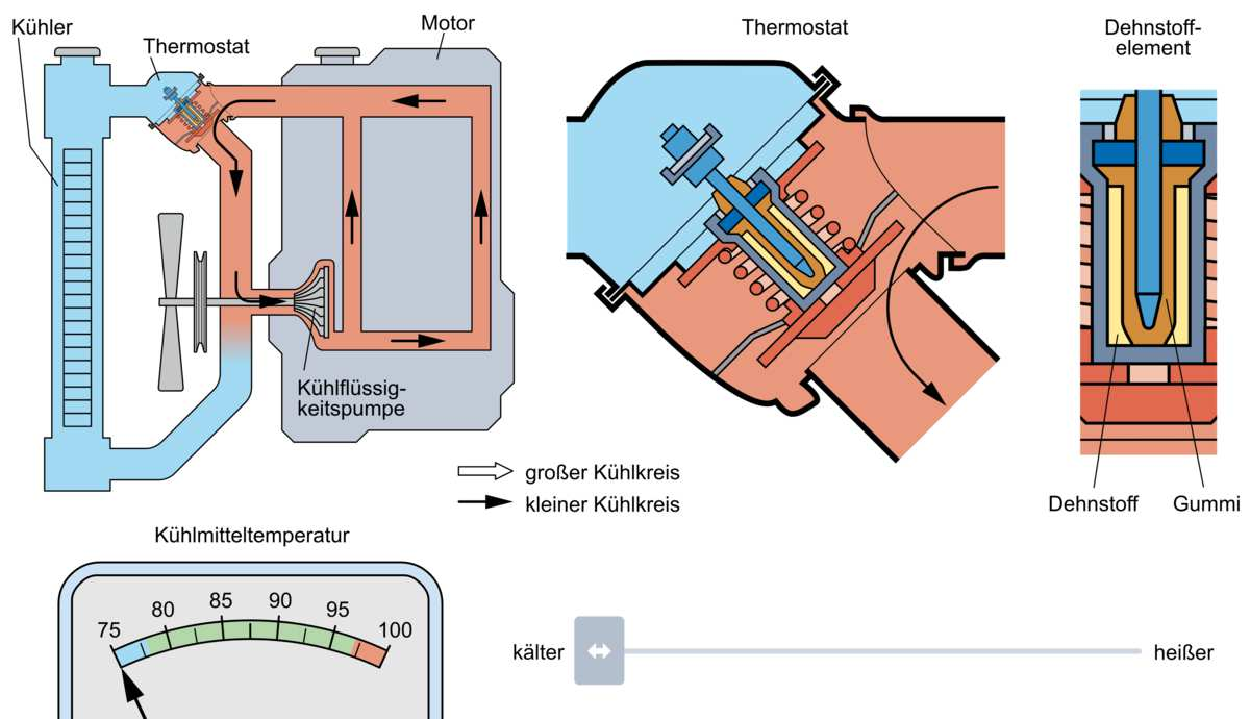
\includegraphics[width=0.5\textwidth]{images/Kuehlsystem/Kuehlsystem-5.pdf}
\caption{Thermostat - kalter Motor, Quelle: Europa-Verlag}
%\label{fig:}%% anpassen
\end{figure}

\begin{figure}[!ht]% hier: !ht
\centering
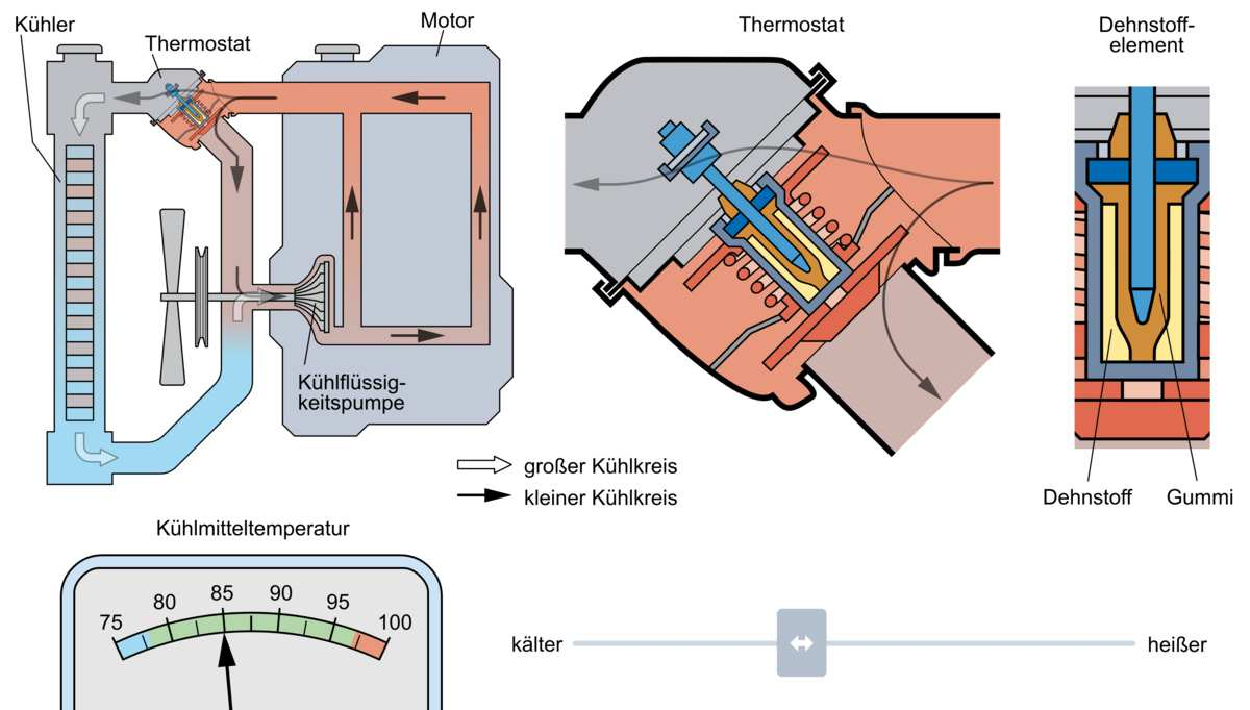
\includegraphics[width=0.5\textwidth]{images/Kuehlsystem/Kuehlsystem-6.pdf}
\caption{Thermostat - Kühlmitteltemperatur $85^\circ\text{C}$, Quelle:
Europa-Verlag}
%\label{fig:}%% anpassen
\end{figure}

\begin{figure}[!ht]% hier: !ht
\centering
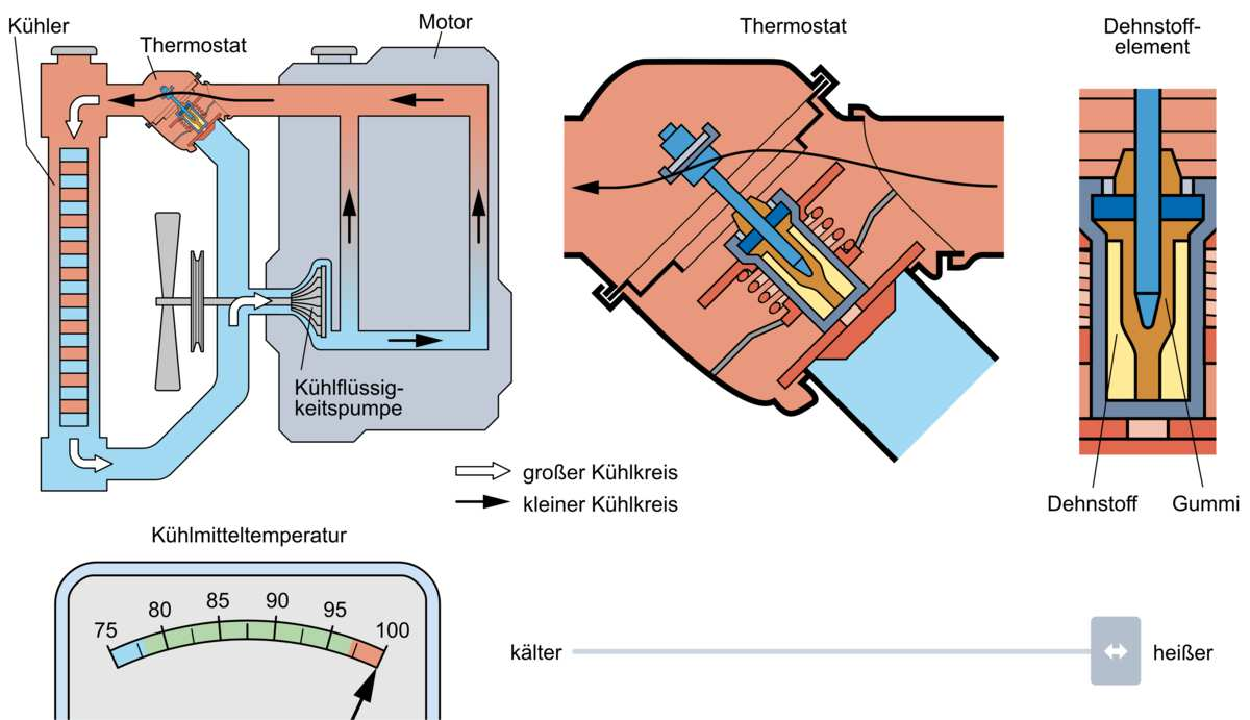
\includegraphics[width=0.5\textwidth]{images/Kuehlsystem/Kuehlsystem-7.pdf}
\caption{Thermostat - heißer Motor, Quelle: Europa-Verlag}
%\label{fig:}%% anpassen
\end{figure}

\begin{enumerate}
\item
  \textbf{Kleiner Kühlkreislauf} (kaltem Motor)

  \begin{itemize}
  \item
    Ventil geschlossen $\to$ kein Durchfluss zum Kühler
  \item
    \emph{Kreislauf:} Kühlmittelpumpe $\to$ Turbolader $\to$ Motor
    $\to$ Thermostat $\to$ Kühlmittelpumpe

    \begin{itemize}
    \item
      Bei Innenraumheizung: einen Teil des erwärmten Kühlmittels wird
      über Heizungswärmetauscher geführt
    \end{itemize}
  \end{itemize}
\item
  \textbf{großer Kühlkreislauf} (Betriebstemperatur)

  \begin{itemize}
  \item
    Ventil öffnet $\to$ Durchfluss zum Kühler (Kühlmitteltemperatur
    etwa $80^\circ\text{C}$)
  \item
    Ventil geöffnet $\to$ voller Durchfluss zum Kühler
    (Kühlmitteltemperatur etwa $95^\circ\text{C}$)
  \item
    \emph{Kreislauf:} Kühlmittelpumpe $\to$ Turbolader $\to$ Motor
    $\to$ Kühler $\to$ Thermostat $\to$ Kühlmittelpumpe
  \end{itemize}
\end{enumerate}

\newpage

\section{Elektronisches Wärmemanagement
(Kennfeldkühlung)}\label{elektronisches-waermemanagement-kennfeldkuehlung}

\begin{figure}[!ht]% hier: !ht
\centering
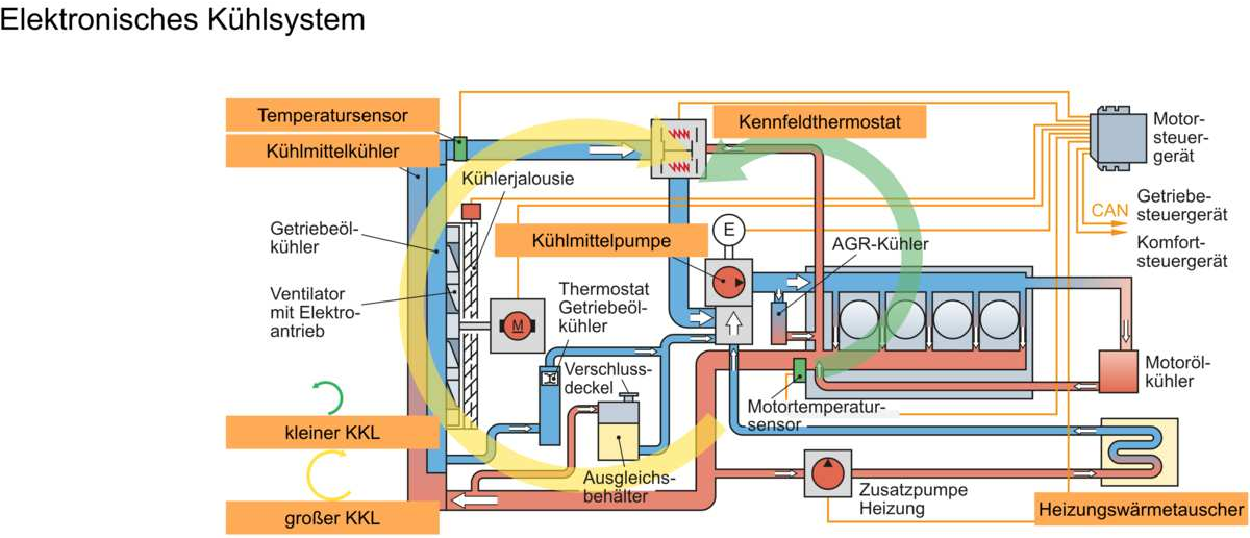
\includegraphics[width=0.7\textwidth]{images/Kuehlsystem/Kuehlsystem-1.pdf}
\caption{Kennfeldkühlung, Quelle: Europa-Verlag}
%\label{fig:}%% anpassen
\end{figure}

zwei Betriebszustände

\begin{enumerate}
\item
  \textbf{Eco-Betrieb - Teillast} (kleiner Kühlkreislauf)

  \begin{itemize}
  \item
    Thermostatheizung: aus
  \item
    Temperatur: bis $106^\circ\text{C}$
  \item
    Warum ist der Motorwirkungsgrad höher?

    \begin{itemize}
    \item
      $\to$ der thermische Wirkungsgrad steigt aufgrund der höheren
      Motortemperatur.
    \end{itemize}
  \end{itemize}
\item
  \textbf{Volllast-Betrieb} (großer Kühlkreislauf)

  \begin{itemize}
  \item
    Thermostatheizung: an
  \item
    Temperatur: $> 90^\circ\text{C}$
  \item
    Wodurch wird ein höherer Füllungsgrad erzielt?

    \begin{itemize}
    \item
      $\to$ kältere Luft hat eine größere Dichte. Die angesaugte
      Luftmasse steigt.
    \end{itemize}
  \item
    Schutz vor Überhitzung der Motorbauteile
  \end{itemize}
\end{enumerate}

\textbf{Ansteuerung Kennfeldthermostat}, die Heizung des Thermostats
wird vom Motorsteuergerät über ein PWM-Signal angesteuert. In
Abhängigkeit von der Pulsweite und Zeit ergibt sich eine
unterschiedliche Aufheizung.

Im Dehnstoffelement ist ein Heizwiderstand eingebettet. Wenn dieser
bestromt wird, erwärmt er das Dehnstoffelement zusätzlich und die
Verstellung erfolgt nun nicht mehr allein in Abhängigkeit von der
Kühlmitteltemperatur, sondern wird vom Motorsteuergerät (nach Kennfeld,
Sollwert) vorgegeben.

\textbf{Wodurch öffnet der Kennfeldthermostat den großen Kühlkreislauf?}

\begin{enumerate}
\item
  \textbf{Eco-Modus}, das Dehnstoffelement wird vom Kühlmittel erwärmt
  und dehnt sich aus. Öffnet erst bei höheren Temperaturen
  $> 106^\circ\text{C}$.
\item
  \textbf{Volllast - Modus}, der Kennfeldthermostat wird über die
  Heizwendel erwärmt. Öffnet schon bei niedrigerer Temperatur
  $> 90^\circ\text{C}$.
\end{enumerate}

\begin{figure}[!ht]% hier: !ht
\centering
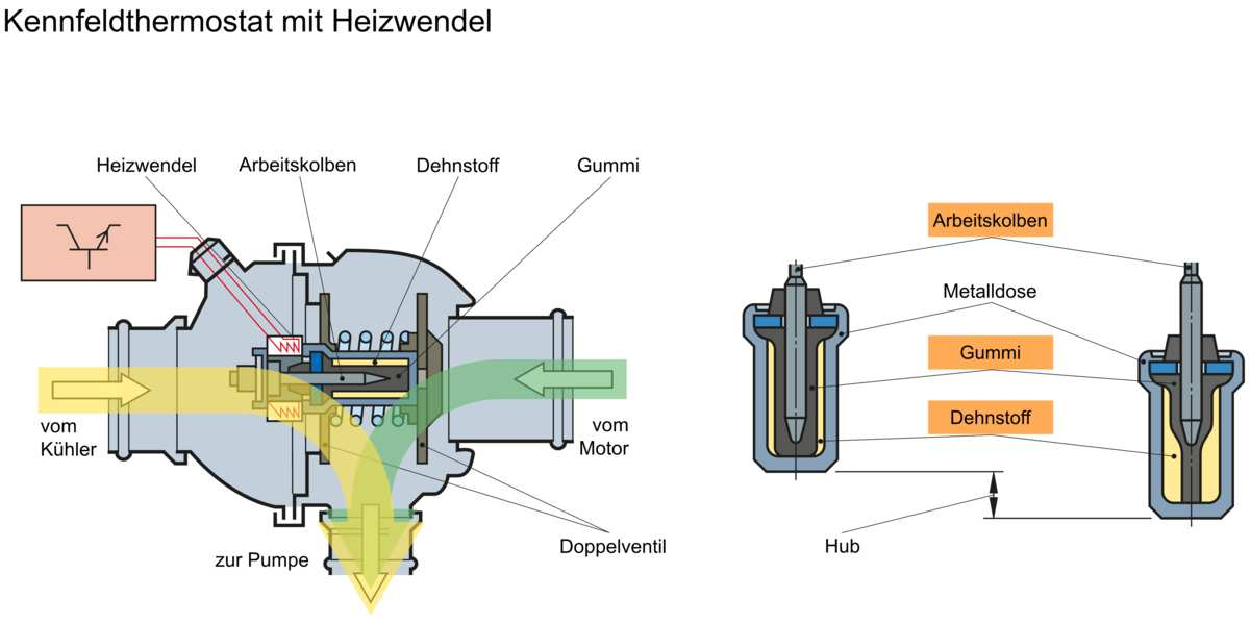
\includegraphics[width=0.6\textwidth]{images/Kuehlsystem/Kuehlsystem-2.pdf}
\caption{Kennfeldthermostat mit Heizwendel, Quelle: Europa-Verlag}
%\label{fig:}%% anpassen
\end{figure}

\newpage

\textbf{Nenne Vorteile der Kennfeldkühlung}

\begin{itemize}
\item
  schnelles Erreichen der Motorbetriebstemperatur und Katalysators
  (Begründung: vgl. Kühlmitteltemperatur bei Teillast)
\item
  Verbesserung der Innenraumheizung
\item
  Motortemperatur / Kühlmitteltemperatur bei Teillast auf bis zu
  $120^\circ\text{C}$ anheben $\to$ bis an die Grenzen der
  Zündfähigkeit

  \begin{itemize}
  \item
    verbesserte Viskosität des Motoröls $\to$ verminderte
    Motorinnenreibung
  \item
    verbesserte Gemischbildung $\to$ durch bessere Verdampfung des
    Kraftstoffs
  \item
    Verbrauchsreduzierung und die Reduzierung der Schadstoffemissionen
  \end{itemize}
\item
  Motortemperatur / Kühlmitteltemperatur bei Volllast senken $\to$
  Schutz vor Überhitzung der Motorbauteile
\end{itemize}

\textbf{Nenne Vorteile einer elektrischen Kühlmittelpumpe}

\begin{enumerate}
\item
  Förderleistung ist unabhängig von der Motordrehzahl
\item
  Pumpe kann zur schnelleren Aufheizung abgeschaltet werden
\item
  Nach Abschalten des Verbrennungsmotors kann die Pumpe weiterlaufen
\item
  Kraftstoff einsparen
\end{enumerate}

\newpage

\section{Antriebsarten von Ventilatoren /
Lüfter}\label{antriebsarten-von-ventilatoren-luefter}

\begin{enumerate}
\item
  \textbf{hydrostatischer Lüfter}
\item
  \textbf{elektrischer Lüfter}
\item
  \textbf{Lüfter mit Viscokupplung} (temperaturabhängige Kupplung,
  Riementrieb)

  \begin{enumerate}
  \def\labelenumii{\arabic{enumii}.}
  \item
    \emph{Kalter Motor}

    \begin{itemize}
    \item
      Bimetallelement verschließt Ventilöffnung
    \item
      Silikonöl wird vom Arbeitsraum in den Vorratsraum gefördert
    \item
      Antriebsscheibe hat keine Verbindung zur Lüfternabe
    \item
      Lüfter ist getrennt
    \end{itemize}
  \item
    \emph{Heißer Motor}

    \begin{itemize}
    \item
      Bimetallelement heizt sich auf und öffnet Ventilöffnung
    \item
      Silikonöl füllt sich in beiden Räumen gleich
    \item
      Kraftfluss wird stufenlos hergestellt zwischen Antriebsscheibe und
      Lüfternabe (zunehmende Reibung des Silikonöls)
    \end{itemize}
  \end{enumerate}

  \begin{itemize}
  \item
    Kühlerabluft trifft auf ein Bimetall, dessen thermische Verformung
    ein Öffnen und Schließen eines Ventils bewirkt. Abhängig von dieser
    Ventilstellung erfolgt die Einstellung der Lüfterdrehzahlen.
  \item
    \emph{Bemerkung:} System arbeitet immer mit Schlupf
    (Flüssigkeits-Haftungsbereich, Drehzahldifferenz), Antriebsscheibe
    dreht mit Riemendrehzahl, Lüfter mit Viscokupplung: nicht legen.
  \end{itemize}
\end{enumerate}

\begin{figure}[!ht]% hier: !ht
\centering
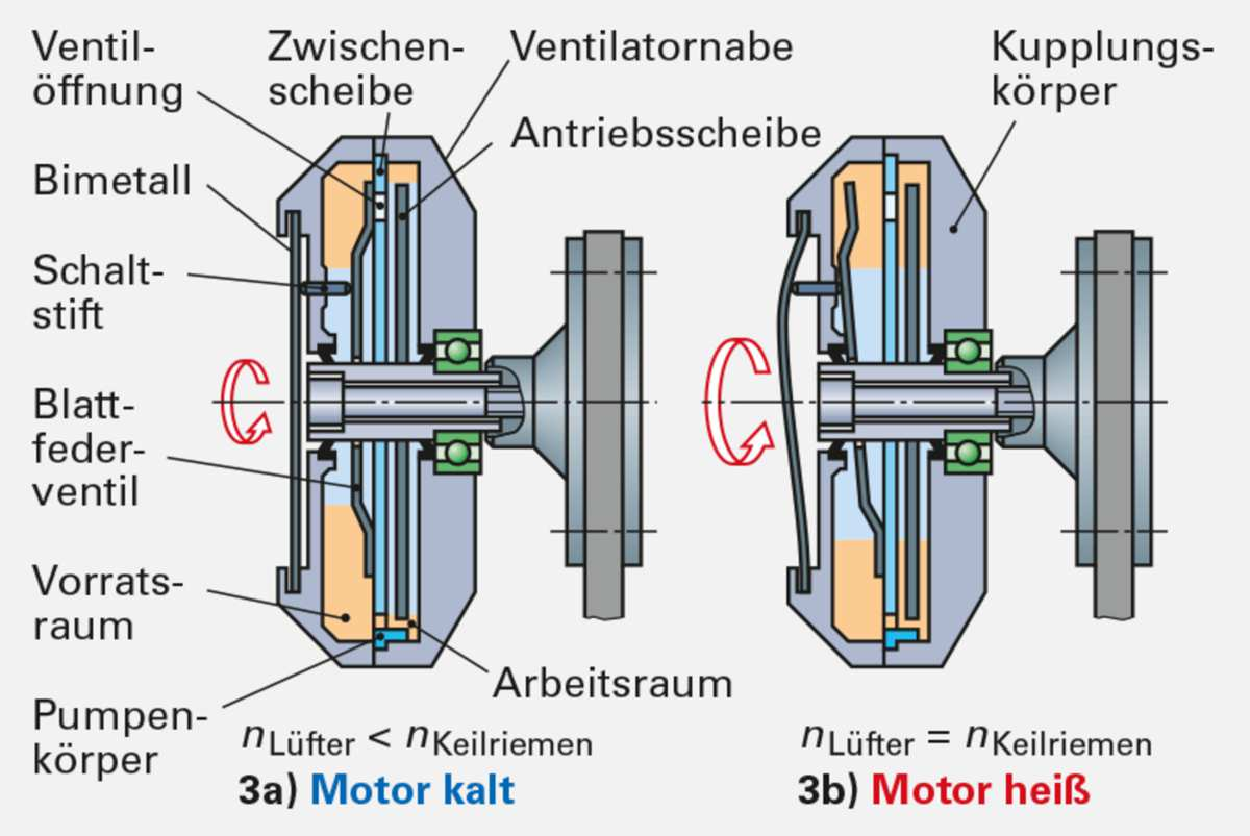
\includegraphics[width=0.5\textwidth]{images/Kuehlsystem/Kuehlsystem-3.pdf}
\caption{Viscokupplung, Quelle: Europa-Verlag}
%\label{fig:}%% anpassen
\end{figure}

\textbf{Aufgabe von Ventilatoren} bei einer bestimmten
Kühlmitteltemperatur eine ausreichende Kühlluftmenge zur Verfügung
stellen, wenn Fahrtwind nicht ausreicht bei Stillstand oder langsame
Fahrt oder Stop-and-Go-Betrieb im Stadtverkehr.

\section{Einfüllverschluss Kühlsystem
(Prüfung)}\label{einfuellverschluss-kuehlsystem-pruefung}

\begin{enumerate}
\item
  \textbf{Überdruckventil} durch den Überdruck kann die
  Kühlmitteltemperatur bis auf $120^\circ\text{C}$ ansteigen, ohne
  dass die Kühlflüssigkeit siedet.
\item
  \textbf{Unterdruckventil} beim Abkühlen der Kühlflüssigkeit tritt
  durch die Volumenverkleinerung ein Unterdruck auf. Durch das öffnende
  Ventil kann der Druck ausgeglichen werden. Dadurch wird verhindert,
  dass sich der Kühler einbeult oder Schläuche zusammenziehen.
\end{enumerate}

\begin{figure}[!ht]% hier: !ht
\centering
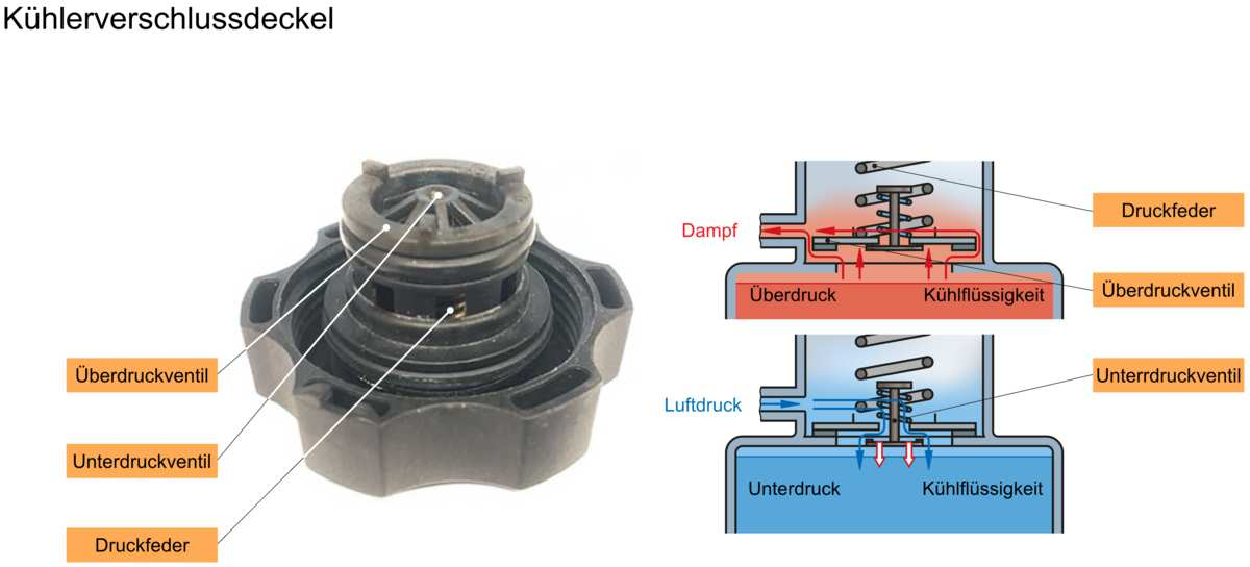
\includegraphics[width=0.7\textwidth]{images/Kuehlsystem/Kuehlsystem-4.pdf}
\caption{Kühlerverschlussdeckel, Quelle: Europa-Verlag}
%\label{fig:}%% anpassen
\end{figure}

\section{Welche Ursachen können zur Überhitzung des Motors führen?
(Motor / Kühlmittel zu
heiß)}\label{welche-ursachen-koennen-zur-ueberhitzung-des-motors-fuehren-motor-kuehlmittel-zu-heiss}

\begin{enumerate}
\item
  Lüftermotor oder Steuerung defekt
\item
  zu wenig Flüssigkeit im System (Kühlmittelverlust)
\item
  Kühllamellen verschmutzt
\item
  Kühler verstopft
\item
  Thermostat öffnet nicht
\item
  Luft im System
\item
  Überdruckventil undicht
\item
  Pumpe defekt
\item
  defekter Keilriemen
\item
  Kennfeldthermostat (Elektrische Anschluss)

  \begin{itemize}
  \item
    Leitungsbruch
  \item
    Übergangswiderstand (korrodierten Stecker) $\to$ Thermostat nicht
    richtig beheizt wird und schnell genug öffnet
  \end{itemize}
\end{enumerate}

\section{Prüfungshinweise zum
Kühlsystem}\label{pruefungshinweise-zum-kuehlsystem}

\begin{enumerate}
\item
  \textbf{Refraktometer}

  \begin{itemize}
  \item
    Dichte Batteriesäure
  \item
    Gefrierpunkt von Kühlmittel

    \begin{itemize}
    \item
      Ethylenglykolbasis G11/12
    \item
      Propylenglykolbasis G13
    \end{itemize}
  \item
    Gefrierpunkt von Scheibenwaschflüssigkeit
  \item
    Harnstoffkonzentration von AdBlue
  \end{itemize}
\item
  \textbf{Dichtheitsprüfung}

  \begin{itemize}
  \item
    Dauer: 2 Minuten
  \item
    Überdruck
  \end{itemize}
\item
  \textbf{$CO_2$-Testgerät}

  \begin{itemize}
  \item
    Undichtigkeiten zwischen Verbrennungsraum und Kühlsystem erkennen
  \end{itemize}
\end{enumerate}

Kühlmittel \emph{nicht} mischen!
